\documentclass{standalone}
\usepackage{tikz}
\begin{document}
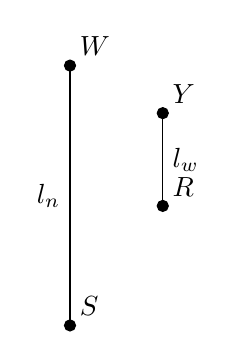
\begin{tikzpicture}[scale=1.0]
  \filldraw (0.0, 0.0) circle (2pt) node[above right] {$S$};
  \filldraw (0.0, 3.3001) circle (2pt) node[above right] {$W$};
  \filldraw (1.1783, 1.5179) circle (2pt) node[above right] {$R$};
  \filldraw (1.1783, 1.5179 + 1.1783) circle (2pt) node[above right] {$Y$};
  \draw (0.0, 0.0) -- (0.0, 3.3001) node[midway, left] {$l_n$};
  \draw (1.1783, 1.5179) -- (1.1783, 1.5179 + 1.1783) node[midway, right] {$l_w$};
\end{tikzpicture}
\end{document}